
\chapter{Introducció a \emph{Machine Learning}}
\section{Introducció}

Tenim N dades i volem ajustar-les a una funció polinòmica de grau M hauríem de crear el següent polinomi:

\[ y(c, x_n) = \sum_{i=0}^{M} c_i·x^i \]

Ja que el nostre objectiu és relacionar una entrada amb una sortida determinada (per exemple en reconeixement facial volem acceptar o denegar l'accés) direm $t_n$ al resultat de la nostra funció d'interpolació que hem de ``deduir".

Així doncs la nostra funció d'error serà la següent:

\[ E(c) = \frac{1}{2} \sum_{n=1}^N (y(c, x_n) - t_n)^2 \]

\subsection{Efecte de N}

\begin{itemize}
	\item Quantes més dades millor
	\item Com que el grau de $M=3$ està inclòs al grau $M=9$, perquè no podem ajustar només al grau 9?
	
	Els coeficients sobrants no tendeixen a 0 necessàriament. Això passarà a mesura que $N \rightarrow \infty$ . Un polinomi que tingui excés de complexitat ($N > 3$) sobreajustarà. El problema del sobreajust es ca solucionant a mesura que N creix.
	
	Per solucionar el problema i escollir la $M$ correcta es generen unes dades de prova i unes dades de comprovació d'error de manera que escollirem la funció que tingui el mínim error.
	
	\begin{figure}[H]
		\centering
		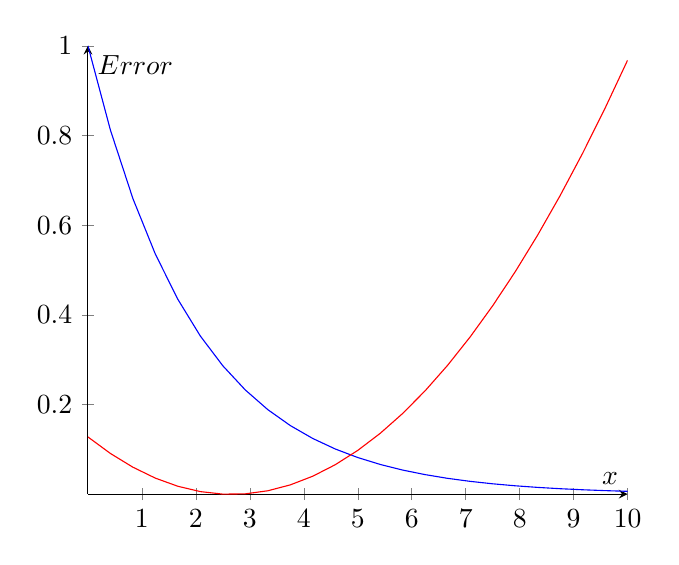
\begin{tikzpicture}
			\begin{axis}[
					xlabel=$x$,
					ylabel=$Error$,
					axis x line=middle,
					axis y line=middle,
					domain=0:10,
					xtick={0, ..., 10}
				]
				\addplot[blue]{exp(-x/2)};
				\addplot[red]{0.002*(3*x-8)^2};
			\end{axis};
		\end{tikzpicture}
	\end{figure}
	
	\item Què hem d'entendre per \textbf{complexitat } d'un model? Si un modelés lineal la seva complexitat és el nombre de coeficients (necessitem una manera de controlar la complexitat) $\rightarrow$ \textbf{Regularització}.
\end{itemize}

\section{Conceptes d'inferència estadística}

$ \mathcal{D} = \{ x_1, ... , x_N \} $ Mostra aleatòria simple:
\begin{itemize}
	\item $X_n$ independents entre si
	\item $X_n$ segueixen la mateixa distribució
\end{itemize}

Cada $x_n (1 \le n \le N)$ és una realització de la v.a. $X_n$

\[ X_n \sim p(x_n, \theta) \]

L'objectiu és trobar una estimació dels paràmetres de $\theta$ basada en $\mathcal{D}$. 

\[ P_n(\mathcal{D}, \theta) = \prod_{n=1}^N p(x_n, \theta) = \mathcal{L}(\theta) \]



\begin{itemize}
	\item La tècnica de \textbf{màxima versemblança} (MV) consisteix en trobar els valors de $\theta$ (diguem-li  $\hat{\theta}$).
	
	\item Definim la funció log-versemblança com $l(\theta) := ln\ \mathcal{L}(\theta) = \sum_{n=1}^{N} ln(p(x_n, \theta))$. 
\end{itemize}
	
\textbf{Exemple} Gaussiana

$$
\text{Equació Gaussiana: } \frac{1}{\sqrt{2\pi\sigma}} exp\left(-\frac{(x_n - \mu)^2}{2\sigma^2}\right)
$$

Primer de tot busquem la funció de log-versemblança $l(\theta) \rightarrow l(\mu, \sigma^2)$. Així doncs, maximitzar $l(\mu, \sigma^2) \leftrightarrow$ minimitzar $-l(\mu, \sigma^2)$

\begin{align*}
	-l(\mu, \sigma^2) &= -\sum_{n=1}^N ln\ p(x_n, \mu, \sigma^2) =  
	-\sum_{n=1}^N ln\left\{ \frac{1}{\sqrt{2\pi\sigma}} exp\left(-\frac{(x_n - \mu)^2}{2\sigma^2}\right) \right\} = \\
	&= \underbrace{\boxed{-\sum_{n=1}^N \left\{ ln(\sqrt{2\pi\sigma}) + 
	\frac{(x_n - \mu)^2}{2\sigma^2} \right\}} }_{\text{Funció } -l(\mu, \sigma^2)}
\end{align*}

Ara busquem $\hat{\mu}$ que és de MV, com que aquest $\hat{\mu}$ fa que $-l(\mu, \sigma^2)$ sigui mínim ho buscarem a partir de la primera derivada.

\begin{align*}
	& \begin{aligned}
		 \textbullet \frac{\partial(-l)}{\partial\mu} &= \sum_{n=1}^N \frac{1}{\sigma^2} (x_n-\mu)(-1) = 0 
		\implies \sum_{n=1}^N (x_n - \mu) = 0 \implies  \\
		& \implies \sum_{n=1}^N x_n = \sum_{n=1}^N \mu \implies \boxed{\hat{\mu} = 
		\frac{1}{N}\sum_{n=1}^N x_n}
	\end{aligned} \\
	& \textbullet \frac{\partial(-l)}{\partial\sigma^2} = \frac{N}{2\sigma^2} - \frac{1}{2\sigma^4}\sum_{n=1}^N (x_n - \mu)^2 = 0
\end{align*}

es substitueix $\mu$ per $\hat{\mu}$ i s'aïlla $\sigma^2 \implies \hat{\sigma}^2 = \frac{1}{N} \sum_{n=1}^N (x_n - \hat{\mu})^2$ 


\subsection{Com de bons són aquests estimadors?}

\begin{itemize}
	\item S'aproximen els valors teòrics $(\mu, \sigma^2)$ quan $N\rightarrow\infty$ ?
	\item Com depèn la qualitat de l'aproximació de N?
	\item Altres estimadors? $\rightarrow$ Quin és el millor?
\end{itemize}

\subsection{Propietats d'un estimador?}

\subsubsection{Unbiasedness}
	
El \textbf{biaix}(BIAS) d'un estimador $\hat{a}$ de $\theta$ és:

$$
\op{bias}(\hat{\theta}) := \mathbb{E}(\hat{\theta}) - \theta
$$

si $bias(\hat{\theta}) = 0$ diem que és no biaixant
	
\subsubsection{Consistency}
	Si es suposa un estimador amb biaix > 0 i aquest es redueix a mesura que $N \to \infty$. Quina \textbf{variabilitat} té?

\subsubsection{Variance}
\textbf{Definició}: la variància d'un estimador $\hat{\theta}$ de $\theta$

$$
\op{Var}(\hat{\theta}) := \mathbb{E}\left[(\hat{\theta} - \mathbb{E}(\hat{\theta}))^2\right]
$$

\textbf{Definició}: direm que un estimador \textbf{és consistent} si

$$
\forall\varepsilon>0, P_n(|\hat{\theta} - \theta| > \epsilon) \rightarrow 0\ quan\ N \to \infty
$$

Si un estimador té $biaix \rightarrow 0;\ var\rightarrow0$ a mesura que $N\rightarrow0$, llavors és consistent.

\textbf{Definició}: L'error quadràtic mitjà(MSE) d'un estimador $\theta\AA$ de $\theta$:
$$
MSE(\hat{\theta}) := \mathbb{E}\left((\hat{\theta}-\theta)^2\right)
$$

\textbf{Teorema}

$$
MSE(\hat{\theta}) = bias^2(\hat{\theta}) + Var(\hat{\theta})
$$


Direm que el millor estimador és aquell que tingui menor MSE. Ens interessen especialment els estimadors sense biaix. Ens interessa aquell que té menor variància. 

\textbf{Definició}: Un estimador és \textbf{eficient} si és no biaixat i té la mínima variància possible.

\textbf{Exemple} (Gaussiana):

$$
\boxed{\hat{\mu}=\frac{1}{N}\sum_{n=1}^N x_n}
$$

\begin{itemize}
	\item $\mathbb{E}(\hat{\mu}) = \mathbb{E}\left(\frac{1}{N}\sum_{n=1}^N X_n\right)=\frac{1}{N}\sum_{n=1}^N \mathbb{E}(X_n) = \frac{1}{N}\sum_{n=1}^N \mu = \frac{1}{N}N\mu = \mu$
	
	\item $\op{Var}(\hat{\mu}) = \op{Var}\left(\frac{1}{N}\sum_{n=1}^N X_n\right) = 
	\frac{1}{N^2}\sum_{n=1}^N Var(X_n) = \frac{1}{N^2}N\sigma^2 = \boxed{ \boldsymbol{\frac{\sigma^2}{N}}}$
	
	\item $\hat{\sigma}^2 = \frac{1}{N}\sum_{n=1}^N(x_n-\hat{\mu})^2$
	
	\item $\mathbb{E}(\hat{\sigma}^2) = \frac{N-1}{N}\sigma^2 \xrightarrow{N\to\infty} \sigma^2$ (biaix és $-\frac{\sigma^2}{N})$
	
	Defineixo $\tilde{\sigma}^2 = \frac{N}{N-1}\hat{\sigma}^2 = \frac{1}{N-1}\sum_{n=1}^N(x_n - \mu)^2 \ \ \  \mathbb{E}(\tilde{\sigma}^2) = \sigma^2$
\end{itemize}


\textbf{Exemple de l'ajust polinòmic (revisitat)}
$$
P_n\left(t_n|x_n, \sigma^2)=\mathcal{N}(t_n, y(x_n, c), \sigma^2\right)
$$

\begin{itemize}
	\item $(x_n, t_n)$ conegudes (D)
	\item $c$ desconegudes (coeficients)
	\item $\sigma^2$ variabilitat estadística (desconeguda)
\end{itemize}